\documentclass[14pt, a4paper]{report}
\usepackage{mathtext}
\usepackage[T2A]{fontenc}
\usepackage[utf8]{inputenc}
\usepackage[russian]{babel}
\usepackage{multirow}
\usepackage{slashbox}
\usepackage{makecell}
\usepackage{graphicx}
\usepackage{physics}
\usepackage{amstext}
\usepackage{caption}
\usepackage{subcaption}

\renewcommand{\thesection}{\arabic{section}.}
\renewcommand{\thesubsection}{\arabic{section}.\arabic{subsection}.}

\title{\textbf{Отчет о выполнении лабораторной работы 2.5.1 "Измерение коэффициента поверхностного натяжения жидкости"}}
\author{Калашников Михаил, Б03-205}
\date{}

\begin{document}
\maketitle

\textbf{Цель работы:}
измерение температурной зависимости коэффициента поверхностного натяжения дистиллированной воды с использованием известного коэффициента поверхностного натяжения спирта; определение полной поверхностной энергии и теплоты, необходимой для изотермического образования единицы поверхности жидкости при различной температуре.
\newline

\textbf{В работе используются:}
\begin{itemize}
\item прибор Ребиндера с термостатом и микроманометром;
\item исследуемые жидкости;
\item стаканы;
\end{itemize}

\section{Теоретические сведения}

Наличие поверхностного слоя приводит к различию давлений по разные стороны от искривленной границы раздела двух сред. Для сферического пузырька с воздухом внутри жидкости избыточное давление даётся формулой Лапласа:
\[\Delta P=P_{внутри}-P_{снаружи}=\frac{2\sigma}{r}\]
где $\sigma$ – коэффициент поверхностного натяжения, $P_{внутри}$ и $P_{снаружи}$ – давление внутри пузырька и снаружи, $r$ -- радиус кривизны поверхности раздела двух фаз.

\section{Экспериментальная установка}

\begin{figure}[!ht]
\centering
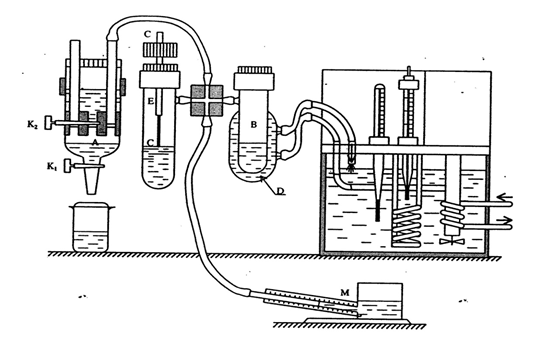
\includegraphics[scale=0.6]{terma7_01.png}
\caption{Схема установки для измерения температурной зависимости коэффициента поверхностного натяжения}
\end{figure}

Исследуемая жидкость (дистиллированная вода) наливается в сосуд В (рис.1). Тестовая жидкость (этиловый спирт) наливается в сосуд Е. При измерениях колбы герметично закрываются пробками. Через одну из двух пробок проходит полая металлическая игла С. Этой пробкой закрывается сосуд, в котором проводятся измерения. Верхний конец иглы открыт в атмосферу, а нижний погружен в жидкость. Другой сосуд герметично закрывается второй пробкой. При создании достаточного разряжения воздуха в колбе с иглой пузырьки воздуха начинают пробулькивать через жидкость. Поверхностное натяжение можно определить по величине разряжения, необходимого для прохождения пузырьков.

Разряжение в системе создается с помощью аспиратора А. Кран К2 разделяет две полости аспиратора. Верхняя полость при закрытом кране К2 заполняется водой. Затем кран К2 открывают и заполняют водой нижнюю полость аспиратора. Разряжение воздуха создается в нижней полости при открывании крана К1, когда вода вытекает из неё по каплям. В колбах В и С, соединённых трубками с нижней полостью аспиратора, создается такое же пониженное давление. Разность давлений в полостях с разряженным воздухом и атмосферой измеряется спиртовым микроманометром.

В ходе работы длина столбика ртути микроманометра связана с давлением формулой $\Delta P=\rho_{сп}gl\sin\alpha=\mu l$, где $\mu=1,573\frac{Па}{мм}$.

\section{Проведение эксперимента}

\begin{enumerate}

\setcounter{enumi}{-1}

\item Зафиксируем температуру в помещении: $t_0=26,0\ ^\circ C$.

\item Проверим герметичность установки. Для этого откроем кран К1 и добьемся пробулькивания пузырьков воздуха в колбе. Отметим показания микроманометра. Закроем кран К1 и прнонаблюдаем за столбиком микроманометра. Он остается неподвижным, следовательно установка герметична.

\item Приступим к измерениям. Вновь откроем кран К1 настолько, чтобы частота падения капель составляла 1 каплю в 5 секунд. 

\item Измерим максимальное давление при пробулькивании пузырьков воздуха через спирт, получим $\Delta P=76,5\pm1,8\ Па$. Определим диаметр иглы по формуле $\Delta P=4\sigma_{сп}/d_0$. Получим $d_0=1,15\pm0,03\ мм$. Диаметр, измеренный с помощью микроскопа равен $d=1,0\pm0,1\ мм$.

\item Аккуратно извлечем иглу, просушим ее от спирта и поместим в колбу с дистиллированной водой. Измерим максимальное давление $P_1=208\pm2\ Па$ при пробулькивании и расстояние между верхним концом иглы и неподвиждной частью установки $h_1=8,0\pm0,5\ мм$. Так же отсюда, зная коэффициент поверхностного натяжения спирта, можно найти значение коэффициента поверхностного натяжения воды по формуле: $\sigma_в=\sigma_{сп}\frac{P_1}{\Delta P}=60\pm3\ \frac{мН}{м}$.

\item Утопим иглу в колбу до щелчка. Аналогично измерим величину $h_2=20,0\pm0,5\ мм$ и давление при пробулькивании $P_2=308\pm2\ Па$. Найдем величину $\Delta h = h_2-h_1=12\pm1\ мм$. Измерения предыдущих трех пунктов занесем в таблицу 1.

\item Снимем температурную зависимость $\sigma(T)$ дистиллированной воды. С помощью термостата нагреем воду в колбе до требуемой температуры, выжидая достаточное для прогрева всего объема воды время. После этого проведем измерение давления. Измерения занесем в таблицу 2.	

\end{enumerate}

\section{Обработка данных}

\begin{enumerate}

\setcounter{enumi}{6}

\item Инструментальная погрешность определения давления равна $\sigma_P=\mu\sigma_l=1,6\ Па$, где $\sigma_l=1\ мм$. Инструментальная погрешность опредления температуры равна $\sigma_t=1 ^\circ C$. Коэффициент поверхностного натяжения может быть рассчитан по формуле:
\[\sigma=(P-\rho_вg\Delta h)\cdot\frac{d}{4}\]
\[\varepsilon_{\sigma}=\sqrt{\frac{\sigma_P^2+(\rho_вg\sigma_h)^2}{(P-\rho_вgh)^2}+\varepsilon_d^2+\varepsilon_{P,\ случ}^2}\]

\item Построив прямую МНК для зависимости $\sigma(T)$ и рассчитав погрешность, получим:
\[\dv{\sigma}{t}=-0,11\pm0,02\ \frac{мН}{м\cdot^\circ C}\]

\item Также построим графики зависимостей теплоты образования единицы поверхности жидкости $q=-T\dv{\sigma}{t}$ и поверхностной энергии единицы площади $u=\sigma-T\dv{\sigma}{t}$ от температуры. 

\item Зная, что $\dv{\lambda}{T}/\lambda=\dv{\sigma}{T}/\sigma$, найдем значение $\dv{\lambda}{T}$:
\[\dv{\lambda}{T}=\frac{\lambda}{\sigma}\dv{\sigma}{T}=-79\pm16\ \frac{Дж}{моль\cdot К}\]

\end{enumerate}

\section{Вывод}

Определенное в ходе работы значение $\dv{\sigma}{t}=-0,11\pm0,02\ \frac{мН}{м\cdot^\circ C}$, отличается от табличного, равного $-0,17\ \frac{мН}{м\cdot^\circ C}$, а табличное значение $\dv{\lambda}{T}=-42\ \frac{Дж}{моль\cdot К}$. Также отличаются значения коэффициента поверхностного натяжения. Вероятно данное расхождение обусловлено попаданием спирта в колбу с водой.

\section{Приложения}

\begin{table}[!ht]
\centering
\makebox[\textwidth][c] {
\begin{tabular}{| c | c | c | c | c | c | c | c | c | c | c |}
\hline
$N$ & 1 & 2 & 3 & 4 & 5 & 6 & 7 & 8 & 9 & 10 \\
\hline
$l_{\Delta P},\ мм$ & 48 & 49 & 49 & 49 & 48 & 49 & 48 & 49 & 48 & 49 \\
$l_{P_1},\ мм$ & 132 & 131 & 131 & 132 & 132 & 133 & 133 & 133 & 134 & 133 \\
$l_{P_2},\ мм$ & 195 & 195 & 195 & 195 & 196 & 196 & 196 & 196 & 196 & 196 \\
\hline
\end{tabular}
}
\caption{Показания микроманометра при измерении диаметра и глубины погружения иглы}
\end{table}

\begin{table}[!ht]
\centering
\makebox[\textwidth][c] {
\begin{tabular}{| c | c | c | c | c | c | c | c | c | c | c | c | c |}
\hline
$t, ^\circ C$ & 25.0 & 30.0 & 33.6 & 35.8 & 38.8 & 41.7 & 44.8 & 47.8 & 50.7 & 53.8 & 56.8 & 59.8 \\
\hline
\multirow{5}{*}{$l,\ мм$} & 197 & 197 & 195 & 194 & 194 & 193 & 192 & 191 & 190 & 189 & 189 & 187 \\
& 198 & 196 & 195 & 195 & 194 & 193 & 192 & 191 & 190 & 189 & 189 & 188 \\
& 198 & 196 & 195 & 194 & 193 & 193 & 192 & 191 & 190 & 189 & 188 & 187 \\
& 197 & 196 & 195 & 194 & 194 & 193 & 192 & 191 & 190 & 190 & 188 & 187 \\
& 196 & 196 & 195 & 194 & 194 & 193 & 192 & 191 & 189 & 190 & 189 & 187 \\
\hline
\end{tabular}
}
\caption{Показания микроманометра при измерении коэффициента поверхностного натяжения дистиллированной воды}
\end{table}

\begin{figure}[!ht]
\centering
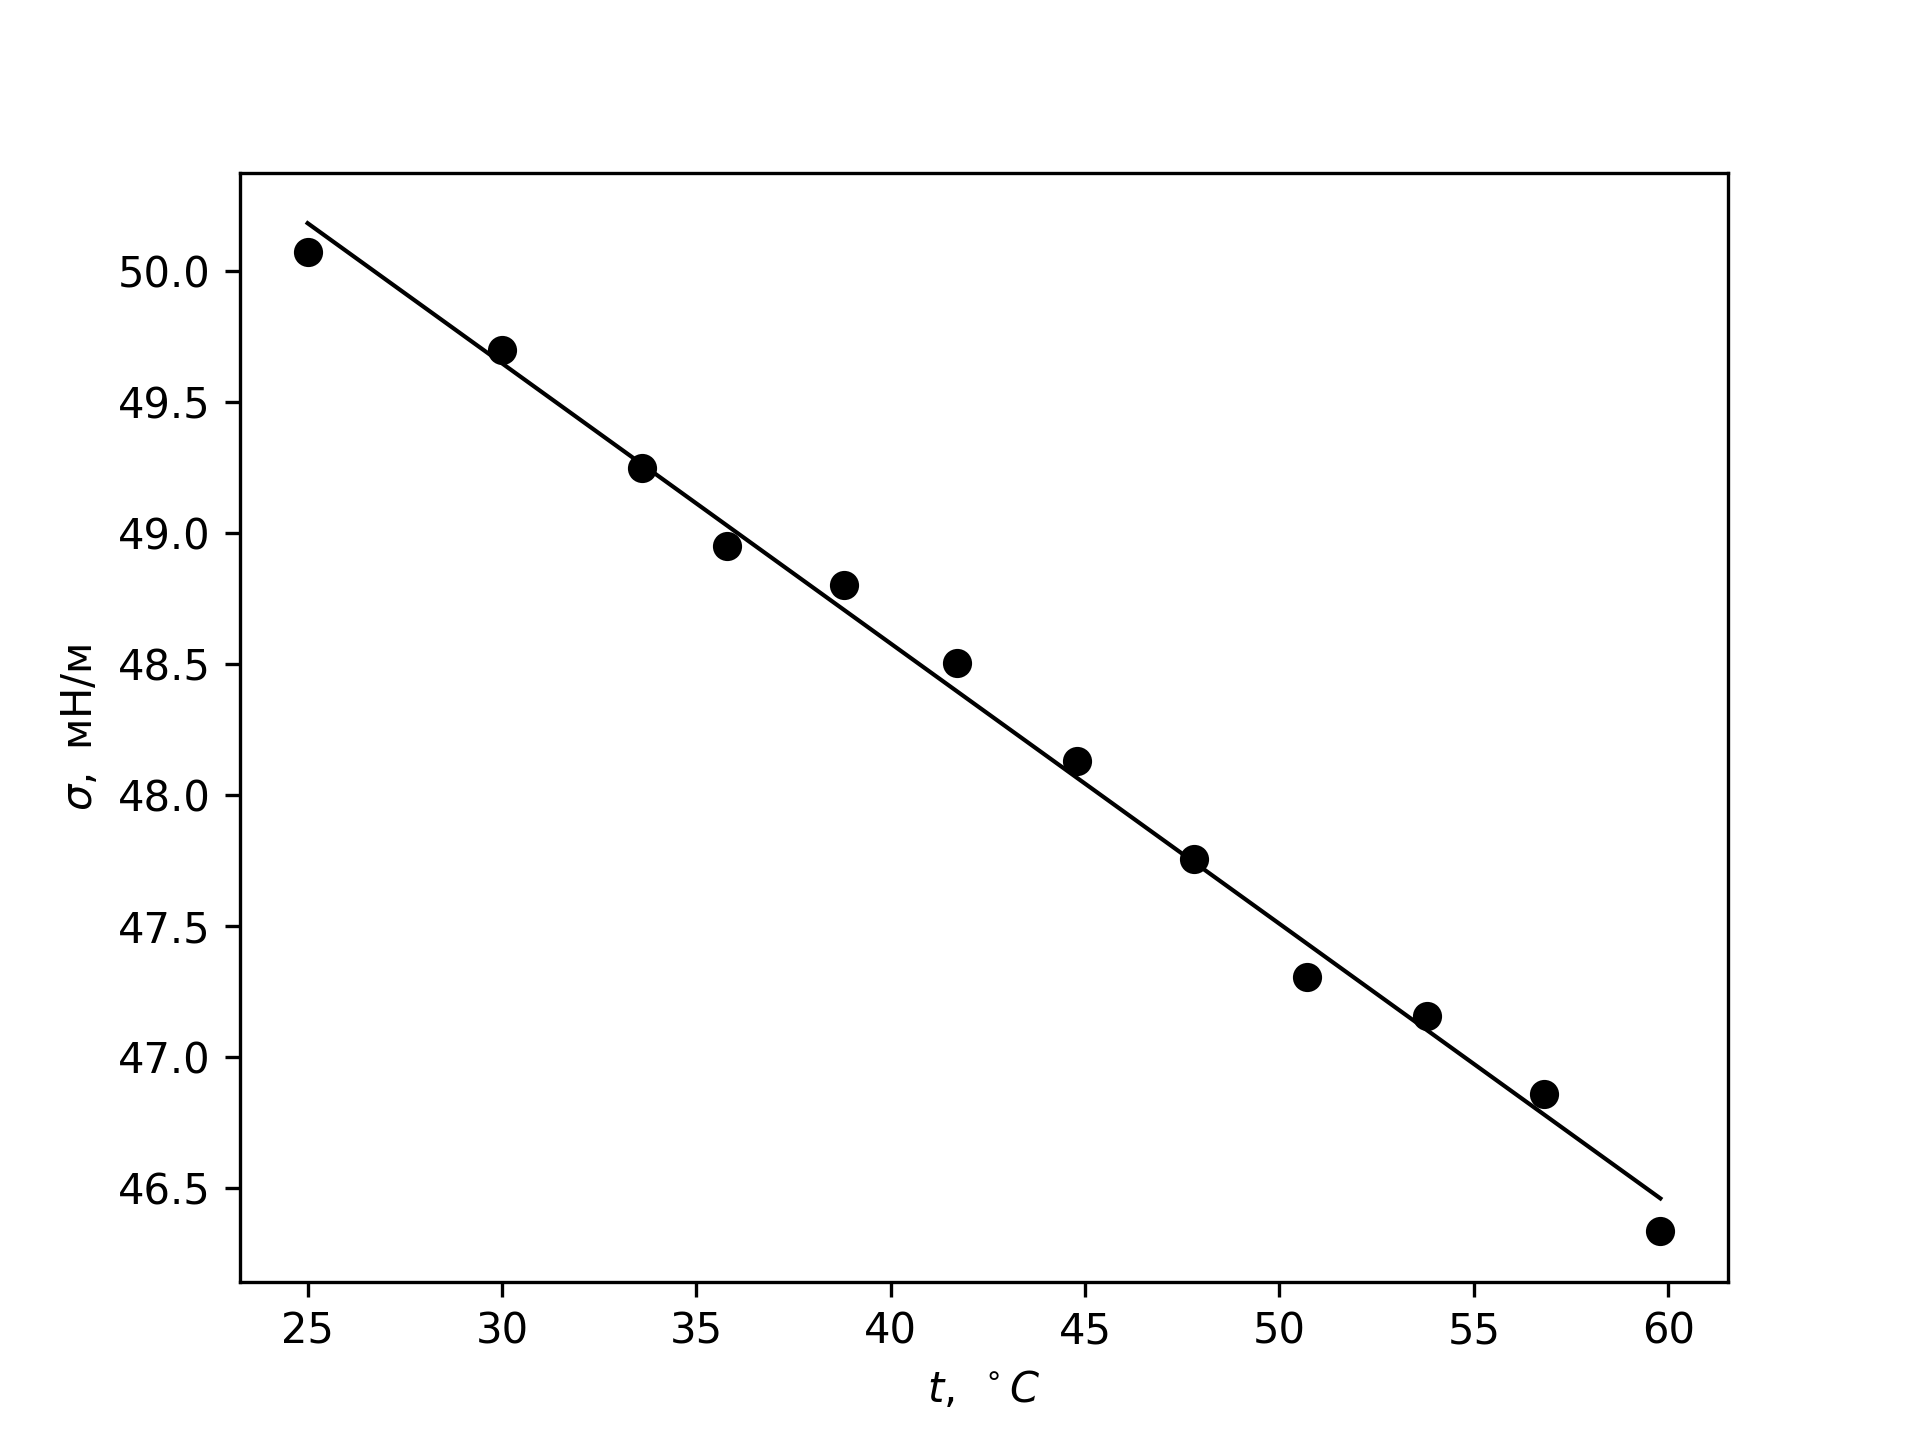
\includegraphics[scale=0.6]{terma7_1.png}
\caption{График зависимости $\sigma(T)$}
\end{figure}

\begin{figure}[!ht]
\centering
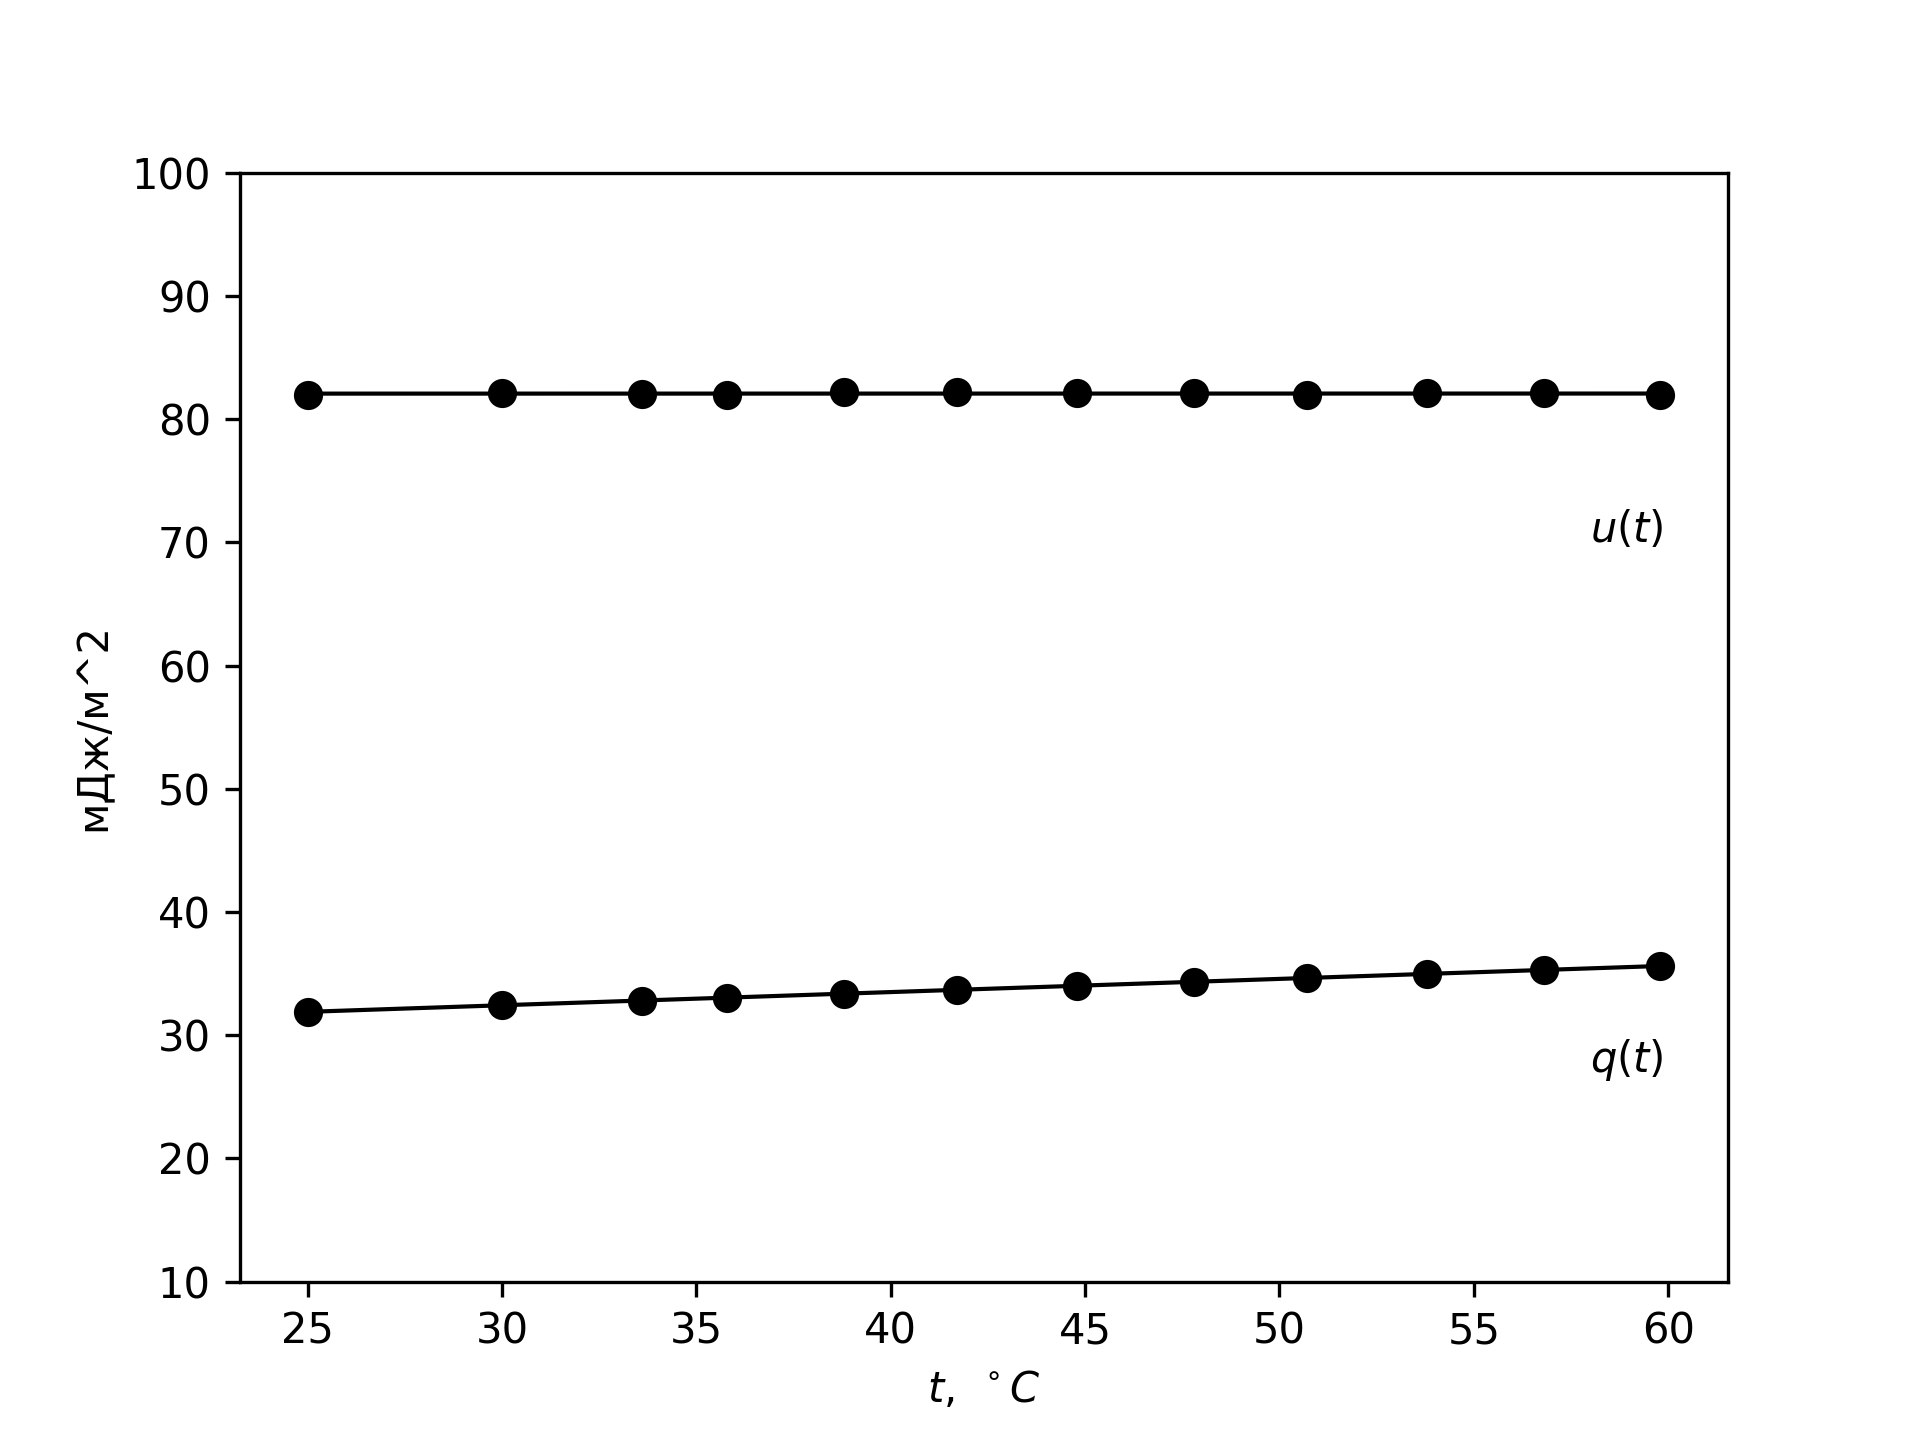
\includegraphics[scale=0.6]{terma7_2.png}
\caption{Графики зависимостей $q(t)$ и $u(t)$}
\end{figure}

\end{document}